
\clearpage
\begin{longtable}{|c|l|l|}
  \endfirsthead
  \hline
  モジュール名                & \multicolumn{2}{l|}{mypage.dart}                                                                                                                    \\ \hline
  モジュール概要               & \multicolumn{2}{p{12cm}|}{マイページ画面を表示するモジュール}                                                                                                        \\ \hline
  責任者                   & \multicolumn{2}{l|}{新谷光城}                                                                                                                           \\ \hline
  \multirow{7}{*}{構成要素} & クラス名                                                                                         & MyPageRouterPage                                     \\ \cline{2-3}
                        & クラス種類                                                                                        & extends AppRouter                                    \\ \cline{2-3}
                        & 処理概要                                                                                         & \multicolumn{1}{p{12cm}|}{MyPageにアクセスするためのRouter}    \\ \cline{2-3}
                        & 入力                                                                                           & なし                                                   \\ \cline{2-3}
                        & 出力                                                                                           & Route                                                \\ \cline{2-3}
                        & \multicolumn{2}{l|}{他クラス・関数との関係}                                                                                                                    \\ \cline{2-3}
                        & \multicolumn{2}{p{14cm}|}{なし}                                                                                                                       \\ \hline
  \multirow{7}{*}{構成要素} & クラス名                                                                                         & MyPage                                               \\ \cline{2-3}
                        & クラス種類                                                                                        & extends StatelessWidget                              \\ \cline{2-3}
                        & 処理概要                                                                                         & \multicolumn{1}{p{12cm}|}{マイページ画面を動的に変更するクラス}        \\ \cline{2-3}
                        & 入力                                                                                           & なし                                                   \\ \cline{2-3}
                        & 出力                                                                                           & Widget                                               \\ \cline{2-3}
                        & \multicolumn{2}{l|}{他クラス・関数との関係}                                                                                                                    \\ \cline{2-3}
                        & \multicolumn{2}{p{14cm}|}{mypage.dartのMyPageStateクラスを組み込む}                                                                                          \\ \hline
  \multirow{7}{*}{構成要素} & クラス名                                                                                         & MyPageState                                          \\ \cline{2-3}
                        & クラス種類                                                                                        & extends StatelessWidget                              \\ \cline{2-3}
                        & 処理概要                                                                                         & \multicolumn{1}{p{12cm}|}{マイページ画面の状態を返すクラス}          \\ \cline{2-3}
                        & 入力                                                                                           & なし                                                   \\ \cline{2-3}
                        & 出力                                                                                           & State                                                \\ \cline{2-3}
                        & \multicolumn{2}{l|}{他クラス・関数との関係}                                                                                                                    \\ \cline{2-3}
                        & \multicolumn{2}{p{14cm}|}{title\_appbar.dartのTitleAppBarクラスを組み込む
  \newline mypage.dartのScrollMyPageDetailクラスを組み込む}                                                                                                                            \\ \hline
  \multirow{7}{*}{構成要素} & クラス名                                                                                         & ScrollMyPageDetail                                   \\ \cline{2-3}
                        & クラス種類                                                                                        & extends StatelessWidget                              \\ \cline{2-3}
                        & 処理概要                                                                                         & \multicolumn{1}{p{12cm}|}{マイページの画面設定一覧スクロールを作成するクラス} \\ \cline{2-3}
                        & 入力                                                                                           & なし                                                   \\ \cline{2-3}
                        & 出力                                                                                           & Widget                                               \\ \cline{2-3}
                        & \multicolumn{2}{l|}{他クラス・関数との関係}                                                                                                                    \\ \cline{2-3}
                        & \multicolumn{2}{p{14cm}|}{change\_general\_corporation.dartのChangeGeneralCorporationクラスを組み込む
  \newline mypage.dartのMyPageListViewクラスを組み込む}                                                                                                                                \\ \hline
  \multirow{7}{*}{構成要素} & クラス名                                                                                         & MyPageListView                                       \\ \cline{2-3}
                        & クラス種類                                                                                        & extends StatelessWidget                              \\ \cline{2-3}
                        & 処理概要                                                                                         & \multicolumn{1}{p{12cm}|}{設定一覧の小分けを作成するクラス}          \\ \cline{2-3}
                        & 入力                                                                                           & \multicolumn{1}{p{12cm}|}{MediaQueryData data,
    \newline ChangeGeneralCorporation store
    \newline List$<$Map$<$String, dynamic$>$$>$
  \newline String}                                                                                                                                                            \\ \cline{2-3}
                        & 出力                                                                                           & Widget                                               \\ \cline{2-3}
                        & \multicolumn{2}{l|}{他クラス・関数との関係}                                                                                                                    \\ \cline{2-3}
                        & \multicolumn{2}{p{14cm}|}{
    change\_general\_corporation.dartのChangeGeneralCorporationクラスを組み込む
    \newline general\_mem\_inf\_conf.dartのGeneralMemInfConfクラスを呼び出し一般会員情報確認画面を表示
    \newline company\_mem\_inf\_conf.dartのCompanyMemInfConfクラスを呼び出し法人会員情報確認画面を表示
    \newline else\_list.dartのElseListクラスを呼び出しお気に入り登録画面、閲覧履歴画面
    \newline apply\_hist.dartのApplyHistクラスを呼び出し応募履歴画面を表示
    \newline not\_post\_list.dartのNotPostListクラスを呼び出し未振り込み投稿一覧画面を表示
    \newline posted\_list.dartのPostedListクラスを呼び出し投稿広告一覧画面を表示
    \newline event\_fee.dartのEventFeeクラスを呼び出しイベント掲載料金プラン画面を表示
    \newline job\_fee.dartのJobFeeクラスを呼び出し求人掲載料金プラン画面を表示
    \newline transfer\_to.dartのTransferToクラスを呼び出し振込先口座番号表示画面を表示
    \newline ask\_page.dartのAskPageクラスを呼び出し問い合わせ画面表示
    \newline rule\_screen.dartのRuleScreenクラスを呼び出し利用規約オーバーレイを表示
    \newline log\_out.dartのLogOutクラスを呼び出しログアウトオーバーレイを表示
    \newline secession.dartのSecessionクラスを呼び出し退会オーバーレイを表示
  }                                                                                                                                                                           \\ \hline
\end{longtable}


\begin{figure}[H]
  \centering
  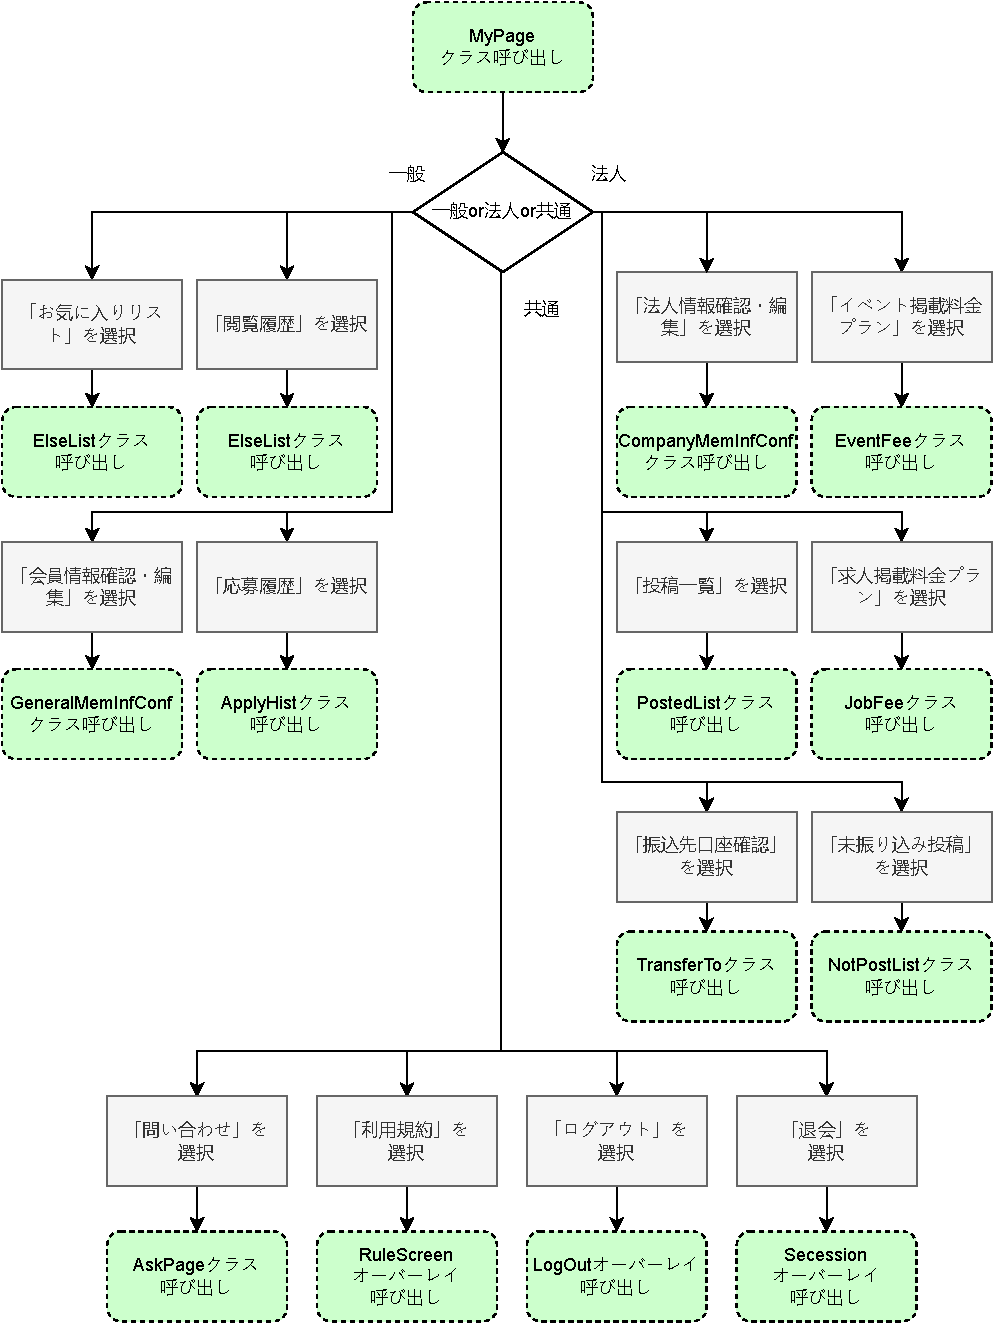
\includegraphics[width=15cm]{./images/internal-design/state_change_diagram/mypage/mypage.pdf}
  \caption{mypage.dartの状態遷移図}
\end{figure}

% \begin{table}[H]
%   \centering
%   \begin{tabular}{|c|l|l|} \hline

%   \end{tabular}
% \end{table}

\begin{table}[H]
  \centering
  \begin{tabular}{|c|l|l|} \hline
    モジュール名                & \multicolumn{2}{l|}{general\_mem\_inf\_conf.dart}                                                                                    \\ \hline
    モジュール概要               & \multicolumn{2}{p{12cm}|}{一般会員情報確認画面を表示するモジュール}                                                                                      \\ \hline
    責任者                   & \multicolumn{2}{l|}{新谷光城}                                                                                                            \\ \hline
    \multirow{7}{*}{構成要素} & クラス名                                                                              & GeneralMemInfConf                                \\ \cline{2-3}
                          & クラス種類                                                                             & extends StatelessWidget                          \\ \cline{2-3}
                          & 処理概要                                                                              & \multicolumn{1}{p{12cm}|}{一般会員情報確認画面を動的に変更するクラス} \\ \cline{2-3}
                          & 入力                                                                                & なし                                               \\ \cline{2-3}
                          & 出力                                                                                & Widget                                           \\ \cline{2-3}
                          & \multicolumn{2}{l|}{他クラス・関数との関係}                                                                                                     \\ \cline{2-3}
                          & \multicolumn{2}{p{14cm}|}{general\_mem\_inf\_conf.dartのGeneralMemInfConfクラスを組み込み}                                                    \\ \hline
    \multirow{7}{*}{構成要素} & クラス名                                                                              & GeneralMemInfConfState                           \\ \cline{2-3}
                          & クラス種類                                                                             & extends StatelessWidget                          \\ \cline{2-3}
                          & 処理概要                                                                              & \multicolumn{1}{p{12cm}|}{一般会員情報確認画面の状態を返すクラス}   \\ \cline{2-3}
                          & 入力                                                                                & なし                                               \\ \cline{2-3}
                          & 出力                                                                                & State                                            \\ \cline{2-3}
                          & \multicolumn{2}{l|}{他クラス・関数との関係}                                                                                                     \\ \cline{2-3}
                          & \multicolumn{2}{p{14cm}|}{
      change\_generalcorporation.dartのChangeGeneralCorporationプロバイダを組み込む
      \newline title\_appbar.dartのTitleAppBarクラスを組み込む
      \newline general\_mem\_inf\_change.dartのGeneralMemInfChangeクラスを呼び出し一般会員情報変更画面を表示
      \newline pass\_change.dartのPassChangeクラスを呼び出しパスワード変更画面を表示
    \newline 戻るボタンの選択で前のモジュールに戻る}                                                                                                                                \\ \hline
  \end{tabular}
\end{table}

\begin{figure}[H]
  \centering
  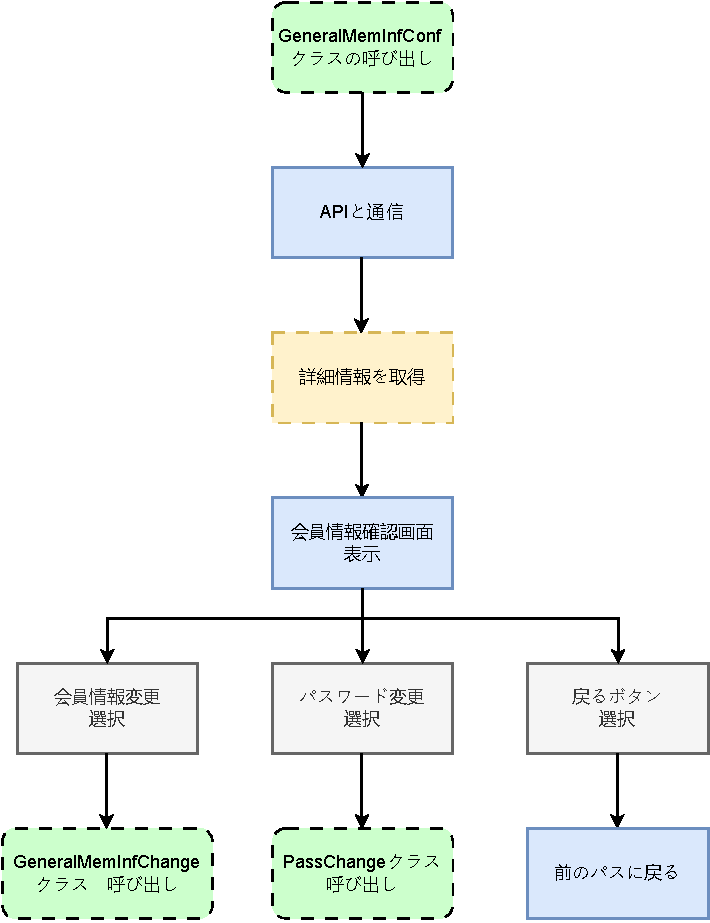
\includegraphics[width=15cm]{./images/internal-design/state_change_diagram/mypage/general_mem_inf_conf.pdf}
  \caption{general\_mem\_inf\_conf.dartの状態遷移図}
\end{figure}

\begin{table}[H]
  \centering
  \begin{tabular}{|c|l|l|} \hline
    モジュール名                & \multicolumn{2}{l|}{general\_mem\_inf\_change.dart}                                                                                           \\ \hline
    モジュール概要               & \multicolumn{2}{p{12cm}|}{一般会員情報変更画面を表示するモジュール}                                                                                               \\ \hline
    責任者                   & \multicolumn{2}{l|}{新谷光城}                                                                                                                     \\ \hline
    \multirow{7}{*}{構成要素} & クラス名                                                                                       & GeneralMemInfChange                              \\ \cline{2-3}
                          & クラス種類                                                                                      & extends StatelessWidget                          \\ \cline{2-3}
                          & 処理概要                                                                                       & \multicolumn{1}{p{12cm}|}{一般会員情報変更画面を動的に変更するクラス} \\ \cline{2-3}
                          & 入力                                                                                         & なし                                               \\ \cline{2-3}
                          & 出力                                                                                         & Widget                                           \\ \cline{2-3}
                          & \multicolumn{2}{l|}{他クラス・関数との関係}                                                                                                              \\ \cline{2-3}
                          & \multicolumn{2}{p{14cm}|}{general\_mem\_inf\_change.dartのGeneralMemInfChangeStateクラスを組み込み}                                                    \\ \hline
    \multirow{7}{*}{構成要素} & クラス名                                                                                       & GeneralMemInfChangeState                         \\ \cline{2-3}
                          & クラス種類                                                                                      & extends StatelessWidget                          \\ \cline{2-3}
                          & 処理概要                                                                                       & \multicolumn{1}{p{12cm}|}{一般会員情報変更画面の状態を返すクラス}   \\ \cline{2-3}
                          & 入力                                                                                         & なし                                               \\ \cline{2-3}
                          & 出力                                                                                         & State                                            \\ \cline{2-3}
                          & \multicolumn{2}{l|}{他クラス・関数との関係}                                                                                                              \\ \cline{2-3}
                          & \multicolumn{2}{p{14cm}|}{
      change\_generalcorporation.dartのChangeGeneralCorporationプロバイダを組み込む
      \newline title\_appbar.dartのTitleAppBarクラスを組み込む
      \newline general\_mem\_inf\_conf.dartのGeneralMemInfConfクラスを呼び出し一般会員情報確認画面を表示
    \newline 戻るボタンの選択で前のモジュールに戻る}                                                                                                                                         \\ \hline
  \end{tabular}
\end{table}

\begin{figure}[H]
  \centering
  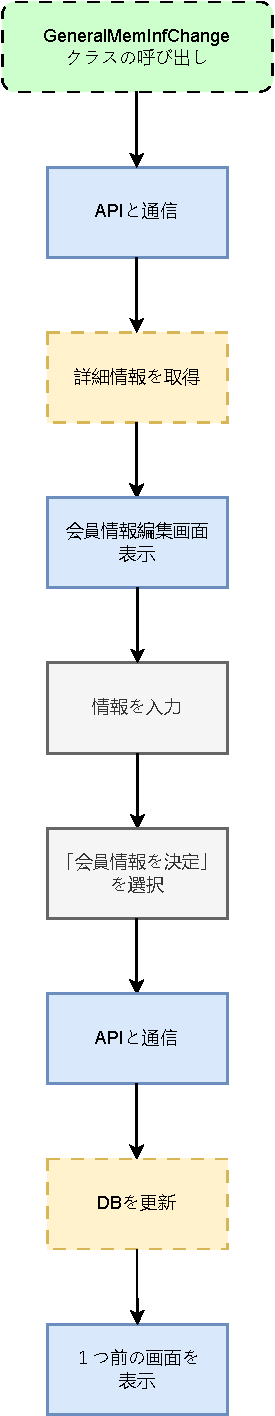
\includegraphics[width=4.5cm]{./images/internal-design/state_change_diagram/mypage/general_mem_inf_change.pdf}
  \caption{general\_mem\_inf\_change.dartの状態遷移図}
\end{figure}

\begin{table}[H]
  \centering
  \begin{tabular}{|c|l|l|} \hline
    モジュール名                & \multicolumn{2}{l|}{apply\_conf.dart}                                                                           \\ \hline
    モジュール概要               & \multicolumn{2}{p{12cm}|}{投稿した求人に応募を行ったユーザの情報を確認する画面を表示するモジュール}                                                 \\ \hline
    責任者                   & \multicolumn{2}{l|}{新谷光城}                                                                                       \\ \hline
    \multirow{7}{*}{構成要素} & クラス名                                                            & ApplyConf                                     \\ \cline{2-3}
                          & クラス種類                                                           & extends StatelessWidget                       \\ \cline{2-3}
                          & 処理概要                                                            & \multicolumn{1}{p{12cm}|}{応募者確認画面を動的に変更するクラス} \\ \cline{2-3}
                          & 入力                                                              & List$<$Map$<$String, dynamic$>$$>$ profiles   \\ \cline{2-3}
                          & 出力                                                              & Widget                                        \\ \cline{2-3}
                          & \multicolumn{2}{l|}{他クラス・関数との関係}                                                                                \\ \cline{2-3}
                          & \multicolumn{2}{p{14cm}|}{ApplyConfStateを組み込む}                                                                  \\ \hline
    \multirow{7}{*}{構成要素} & クラス名                                                            & ApplyConfState                                \\ \cline{2-3}
                          & クラス種類                                                           & extends StatelessWidget                       \\ \cline{2-3}
                          & 処理概要                                                            & \multicolumn{1}{p{12cm}|}{応募者確認画面の状態を返すクラス}   \\ \cline{2-3}
                          & 入力                                                              & なし                                            \\ \cline{2-3}
                          & 出力                                                              & State                                         \\ \cline{2-3}
                          & \multicolumn{2}{l|}{他クラス・関数との関係}                                                                                \\ \cline{2-3}
                          & \multicolumn{2}{p{14cm}|}{
      ApplyConfStateを組み込む
      \newline conf\_conf.dartのConfConfクラスを呼び出し確認確認オーバーレイを表示
    \newline 戻るボタンの選択で前のモジュールに戻る}                                                                                                           \\ \hline
  \end{tabular}
\end{table}

\begin{figure}[H]
  \centering
  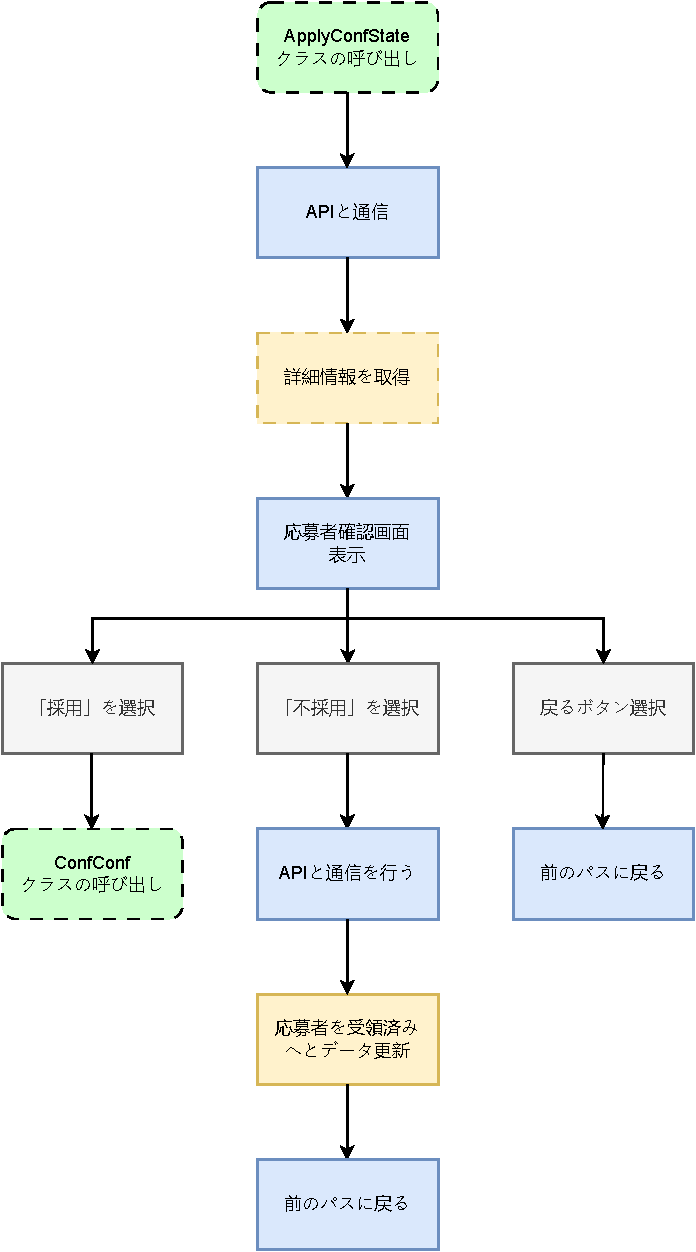
\includegraphics[width=14cm]{./images/internal-design/state_change_diagram/mypage/apply_conf.pdf}
  \caption{apply\_conf.dartの状態遷移図}
\end{figure}

\begin{table}[H]
  \centering
  \begin{tabular}{|c|l|l|} \hline
    モジュール名                & \multicolumn{2}{l|}{transfer\_to.dart}                                                        \\ \hline
    モジュール概要               & \multicolumn{2}{p{12cm}|}{振込先口座表示画面を表示するモジュール}                                                \\ \hline
    責任者                   & \multicolumn{2}{l|}{新谷光城}                                                                     \\ \hline
    \multirow{7}{*}{構成要素} & クラス名                                           & TransferTo                                   \\ \cline{2-3}
                          & クラス種類                                          & extends StatelessWidget                      \\ \cline{2-3}
                          & 処理概要                                           & \multicolumn{1}{p{12cm}|}{振込先口座表示番号を表示するクラス} \\ \cline{2-3}
                          & 入力                                             & なし                                           \\ \cline{2-3}
                          & 出力                                             & Widget                                       \\ \cline{2-3}
                          & \multicolumn{2}{l|}{他クラス・関数との関係}                                                              \\ \cline{2-3}
                          & \multicolumn{2}{p{14cm}|}{戻るボタンの選択で前のモジュールに戻る}                                                \\ \hline
  \end{tabular}
\end{table}

\begin{figure}[H]
  \centering
  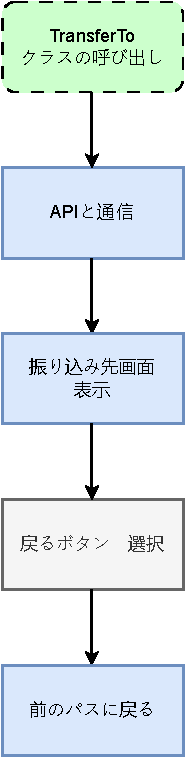
\includegraphics[width=4.5cm]{./images/internal-design/state_change_diagram/mypage/transfer_to.pdf}
  \caption{transfer\_to.dartの状態遷移図}
\end{figure}


\begin{table}[H]
  \centering
  \begin{tabular}{|c|l|l|} \hline
    モジュール名                & \multicolumn{2}{l|}{company\_mem\_inf\_conf.dart}                                                                                    \\ \hline
    モジュール概要               & \multicolumn{2}{p{12cm}|}{法人会員情報確認画面を表示するモジュール}                                                                                      \\ \hline
    責任者                   & \multicolumn{2}{l|}{新谷光城}                                                                                                            \\ \hline
    \multirow{7}{*}{構成要素} & クラス名                                                                              & CompanyMemInfConf                                \\ \cline{2-3}
                          & クラス種類                                                                             & extends StatelessWidget                          \\ \cline{2-3}
                          & 処理概要                                                                              & \multicolumn{1}{p{12cm}|}{法人会員情報確認画面を動的に変更するクラス} \\ \cline{2-3}
                          & 入力                                                                                & なし                                               \\ \cline{2-3}
                          & 出力                                                                                & Widget                                           \\ \cline{2-3}
                          & \multicolumn{2}{l|}{他クラス・関数との関係}                                                                                                     \\ \cline{2-3}
                          & \multicolumn{2}{p{14cm}|}{company\_mem\_inf\_conf.dartのGeneralMemInfConfクラスを組み込み}                                                    \\ \hline
    \multirow{7}{*}{構成要素} & クラス名                                                                              & CompanyMemInfConfState                           \\ \cline{2-3}
                          & クラス種類                                                                             & extends StatelessWidget                          \\ \cline{2-3}
                          & 処理概要                                                                              & \multicolumn{1}{p{12cm}|}{法人会員情報確認画面の状態を返すクラス}   \\ \cline{2-3}
                          & 入力                                                                                & なし                                               \\ \cline{2-3}
                          & 出力                                                                                & State                                            \\ \cline{2-3}
                          & \multicolumn{2}{l|}{他クラス・関数との関係}                                                                                                     \\ \cline{2-3}
                          & \multicolumn{2}{p{14cm}|}{
      change\_generalcorporation.dartのChangeGeneralCorporationプロバイダを組み込む
      \newline title\_appbar.dartのTitleAppBarクラスを組み込む
      \newline cmopany\_mem\_inf\_change.dartのCompanyMemInfChangeクラスを呼び出し法人会員情報変更画面を表示
      \newline pass\_change.dartのPassChangeクラスを呼び出しパスワード変更画面を表示
    \newline 戻るボタンの選択で前のモジュールに戻る}                                                                                                                                \\ \hline
  \end{tabular}
\end{table}

\begin{figure}[H]
  \centering
  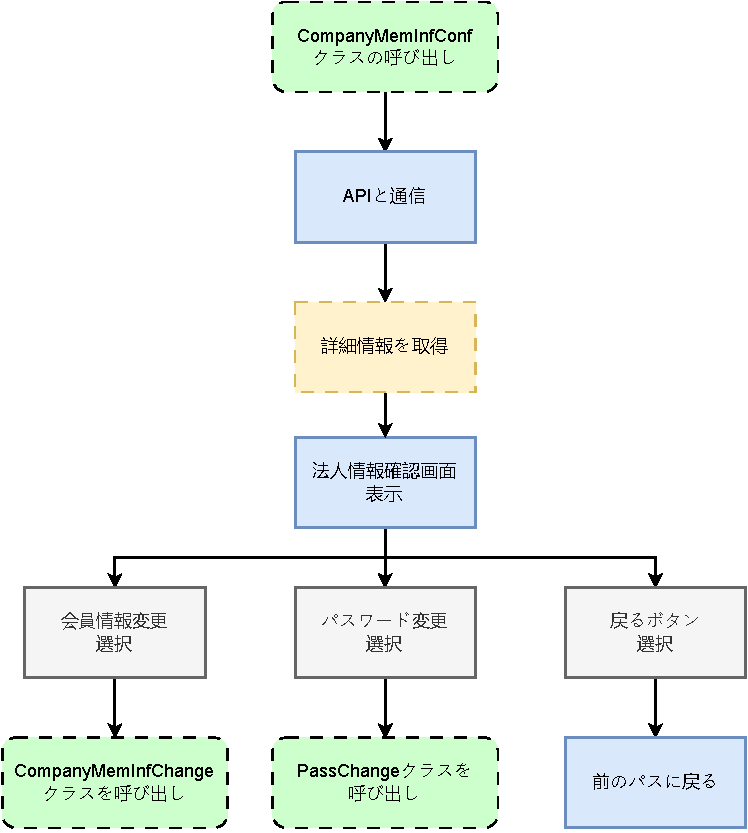
\includegraphics[width=17cm]{./images/internal-design/state_change_diagram/mypage/company_mem_inf_conf.pdf}
  \caption{company\_mem\_inf\_conf.dartの状態遷移図}
\end{figure}


\begin{table}[H]
  \centering
  \begin{tabular}{|c|l|l|} \hline
    モジュール名                & \multicolumn{2}{l|}{company\_mem\_inf\_change.dart}                                                                                      \\ \hline
    モジュール概要               & \multicolumn{2}{p{12cm}|}{法人会員情報編集画面を表示するモジュール}                                                                                          \\ \hline
    責任者                   & \multicolumn{2}{l|}{山本昇永}                                                                                                                \\ \hline
    \multirow{7}{*}{構成要素} & クラス名                                                                                  & CompanyMemInfChange                              \\ \cline{2-3}
                          & クラス種類                                                                                 & extends StatelessWidget                          \\ \cline{2-3}
                          & 処理概要                                                                                  & \multicolumn{1}{p{12cm}|}{法人会員情報編集画面を動的に変更するクラス} \\ \cline{2-3}
                          & 入力                                                                                    & なし                                               \\ \cline{2-3}
                          & 出力                                                                                    & Widget                                           \\ \cline{2-3}
                          & \multicolumn{2}{l|}{他クラス・関数との関係}                                                                                                         \\ \cline{2-3}
                          & \multicolumn{2}{p{14cm}|}{company\_mem\_inf\_change.dartのGeneralMemInfChangeクラスを組み込み}                                                    \\ \hline
    \multirow{7}{*}{構成要素} & クラス名                                                                                  & CompanyMemInfChangeState                         \\ \cline{2-3}
                          & クラス種類                                                                                 & extends StatelessWidget                          \\ \cline{2-3}
                          & 処理概要                                                                                  & \multicolumn{1}{p{12cm}|}{法人会員情報編集画面の状態を返すクラス}   \\ \cline{2-3}
                          & 入力                                                                                    & なし                                               \\ \cline{2-3}
                          & 出力                                                                                    & State                                            \\ \cline{2-3}
                          & \multicolumn{2}{l|}{他クラス・関数との関係}                                                                                                         \\ \cline{2-3}
                          & \multicolumn{2}{p{14cm}|}{
      change\_generalcorporation.dartのChangeGeneralCorporationプロバイダを組み込む
      \newline title\_appbar.dartのTitleAppBarクラスを組み込む
      \newline company\_form.dartのCompanyFormクラスを組み込む
    \newline 戻るボタンの選択で前のモジュールに戻る}                                                                                                                                    \\ \hline
  \end{tabular}
\end{table}

\begin{figure}[H]
  \centering
  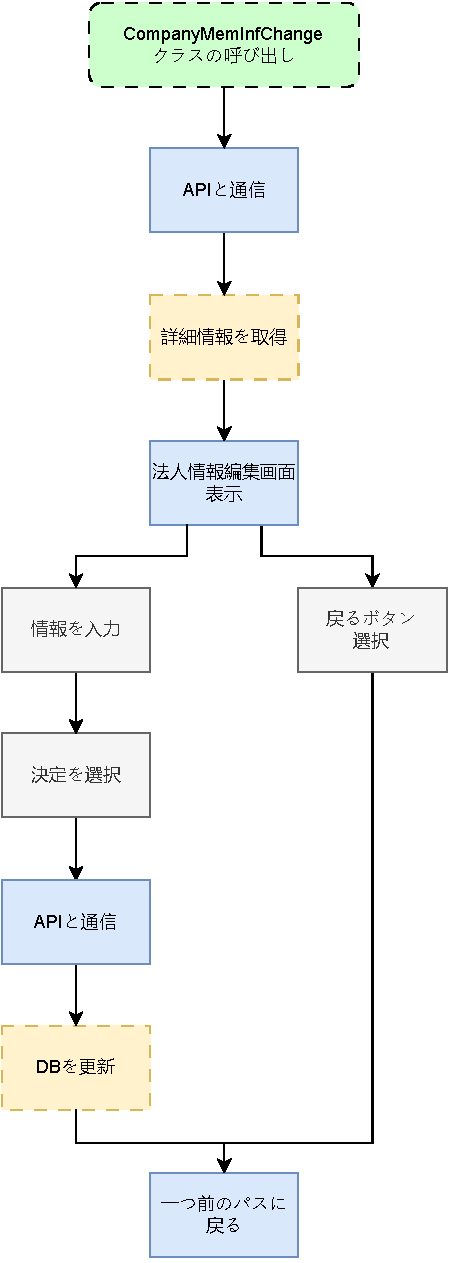
\includegraphics[width=9cm]{./images/internal-design/state_change_diagram/mypage/company_mem_inf_change.pdf}
  \caption{company\_mem\_inf\_change.dartの状態遷移図}
\end{figure}

\begin{table}[H]
  \centering
  \begin{tabular}{|c|l|l|} \hline
    モジュール名                & \multicolumn{2}{l|}{event\_fee.dart}                                                                   \\ \hline
    モジュール概要               & \multicolumn{2}{p{12cm}|}{イベント広告の掲載料金プランを表示するモジュール}                                                    \\ \hline
    責任者                   & \multicolumn{2}{l|}{新谷光城}                                                                              \\ \hline
    \multirow{7}{*}{構成要素} & クラス名                                                & EventFee                                         \\ \cline{2-3}
                          & クラス種類                                               & extends StatelessWidget                          \\ \cline{2-3}
                          & 処理概要                                                & \multicolumn{1}{p{12cm}|}{イベント広告掲載料金プランを表示するクラス} \\ \cline{2-3}
                          & 入力                                                  & なし                                               \\ \cline{2-3}
                          & 出力                                                  & Widget                                           \\ \cline{2-3}
                          & \multicolumn{2}{l|}{他クラス・関数との関係}                                                                       \\ \cline{2-3}
                          & \multicolumn{2}{p{14cm}|}{
      change\_generalcorporation.dartのChangeGeneralCorporationプロバイダを組み込む
      \newline event\_fee\_select.dartのEventPostInfoプロバイダを組み込む
      \newline title\_appbar.dartのTitleAppBarクラスを組み込む
      \newline transfer\_to.dartのTransferToクラスを呼び出し振込口座確認画面を表示
      \newline 戻るボタンの選択で前のモジュールに戻る
    }                                                                                                                              \\ \hline
  \end{tabular}
\end{table}

\begin{figure}[H]
  \centering
  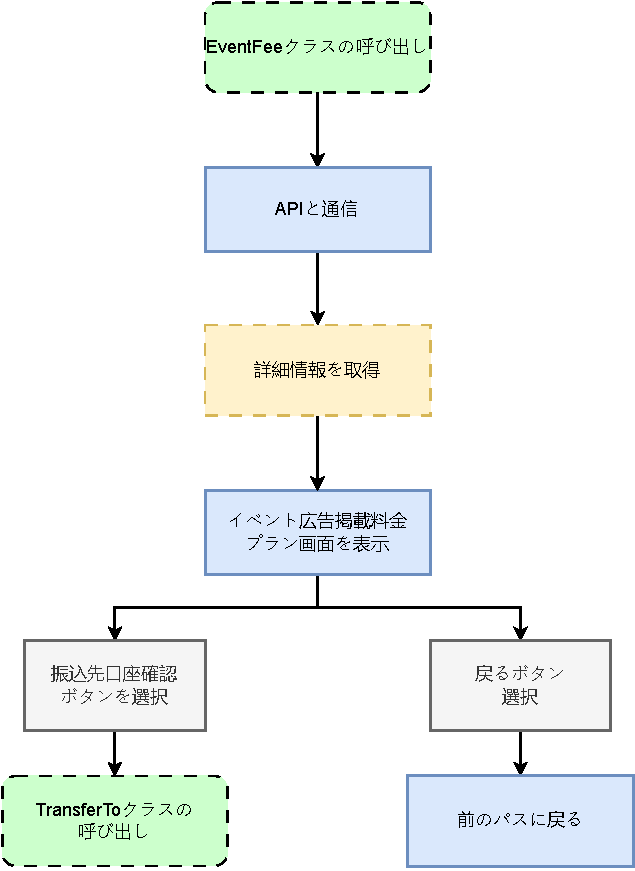
\includegraphics[width=12cm]{./images/internal-design/state_change_diagram/mypage/event_fee.pdf}
  \caption{event\_fee.dartの状態遷移図}
\end{figure}



\begin{table}[H]
  \centering
  \begin{tabular}{|c|l|l|} \hline
    モジュール名                & \multicolumn{2}{l|}{event\_fee\_select.dart}                                                                \\ \hline
    モジュール概要               & \multicolumn{2}{p{12cm}|}{イベント掲載料金プランを選択する画面を表示するモジュール}                                                     \\ \hline
    責任者                   & \multicolumn{2}{l|}{新谷光城}                                                                                   \\ \hline
    \multirow{7}{*}{構成要素} & クラス名                                                    & EventFeeSelect                                    \\ \cline{2-3}
                          & クラス種類                                                   & extends StatelessWidget                           \\ \cline{2-3}
                          & 処理概要                                                    & \multicolumn{1}{p{12cm}|}{求人掲載料金プラン選択画面を表示するクラス}  \\ \cline{2-3}
                          & 入力                                                      & なし                                                \\ \cline{2-3}
                          & 出力                                                      & Widget                                            \\ \cline{2-3}
                          & \multicolumn{2}{l|}{他クラス・関数との関係}                                                                            \\ \cline{2-3}
                          & \multicolumn{2}{p{14cm}|}{
      change\_generalcorporation.dartのChangeGeneralCorporationプロバイダを組み込む
      \newline event\_fee\_select.dartのEventPostInfoプロバイダを組み込む
      \newline title\_appbar.dartのTitleAppBarクラスを組み込む
      \newline job\_post\_write.dartのJobPostWriteクラスを呼び出し求人広告掲載内容記述画面を表示
    \newline 戻るボタンの選択で前のモジュールに戻る}                                                                                                       \\ \hline
    \multirow{7}{*}{構成要素} & クラス名                                                    & EventPostInfo                                     \\ \cline{2-3}
                          & クラス種類                                                   & ChangeNotifier                                    \\ \cline{2-3}
                          & 処理概要                                                    & \multicolumn{1}{p{12cm}|}{イベント広告投稿内容を保存しておくプロバイダ} \\ \cline{2-3}
                          & 入力                                                      & なし                                                \\ \cline{2-3}
                          & 出力                                                      & なし                                                \\ \cline{2-3}
                          & \multicolumn{2}{l|}{他クラス・関数との関係}                                                                            \\ \cline{2-3}
                          & \multicolumn{2}{p{14cm}|}{なし}                                                                               \\ \hline
  \end{tabular}
\end{table}

\begin{figure}[H]
  \centering
  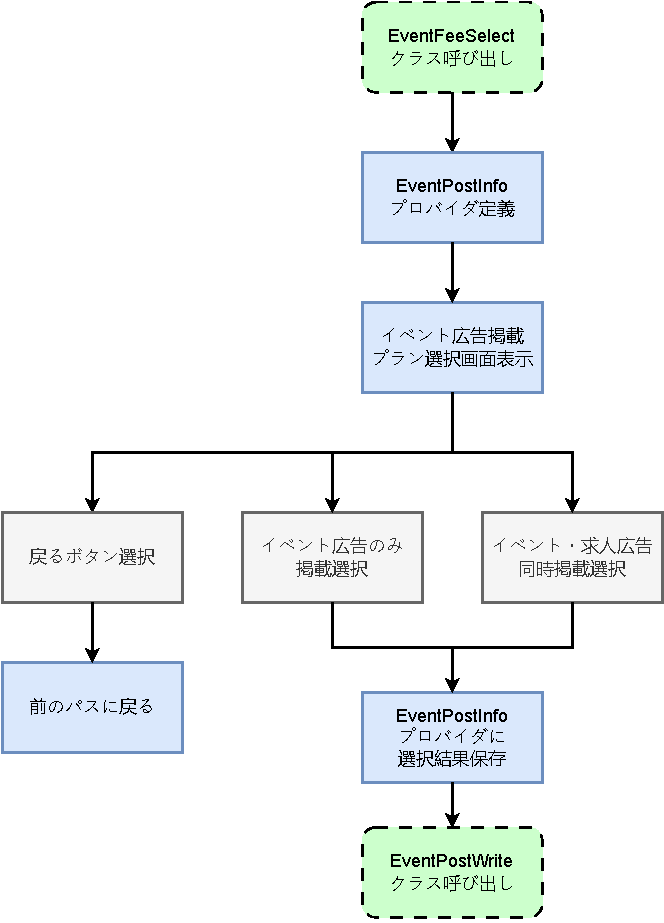
\includegraphics[width=15cm]{./images/internal-design/state_change_diagram/mypage/event_fee_select.pdf}
  \caption{event\_fee\_select.dartの状態遷移図}
\end{figure}

\begin{table}[H]
  \centering
  \begin{tabular}{|c|l|l|} \hline
    モジュール名                & \multicolumn{2}{l|}{job\_fee.dart}                                                                \\ \hline
    モジュール概要               & \multicolumn{2}{p{12cm}|}{求人広告の掲載料金プランを表示するレイヤー}                                                  \\ \hline
    責任者                   & \multicolumn{2}{l|}{新谷光城}                                                                         \\ \hline
    \multirow{7}{*}{構成要素} & クラス名                                             & JobFee                                         \\ \cline{2-3}
                          & クラス種類                                            & extends StatelessWidget                        \\ \cline{2-3}
                          & 処理概要                                             & \multicolumn{1}{p{12cm}|}{求人広告掲載料金プランを表示するクラス} \\ \cline{2-3}
                          & 入力                                               & 契約希望月(int)                                     \\ \cline{2-3}
                          & 出力                                               & Widget                                         \\ \cline{2-3}
                          & \multicolumn{2}{l|}{他クラス・関数との関係}                                                                  \\ \cline{2-3}
                          & \multicolumn{2}{p{14cm}|}{
      change\_generalcorporation.dartのChangeGeneralCorporationプロバイダを組み込む
      \newline job\_fee\_select.dartのJobPostInfoプロバイダを組み込む
      \newline title\_appbar.dartのTitleAppBarクラスを組み込む
      \newline transfer\_to.dartのTransferToクラスを呼び出し振込口座確認画面を表示
      \newline 戻るボタンの選択で前のモジュールに戻る
    }                                                                                                                         \\ \hline
  \end{tabular}
\end{table}

\begin{figure}[H]
  \centering
  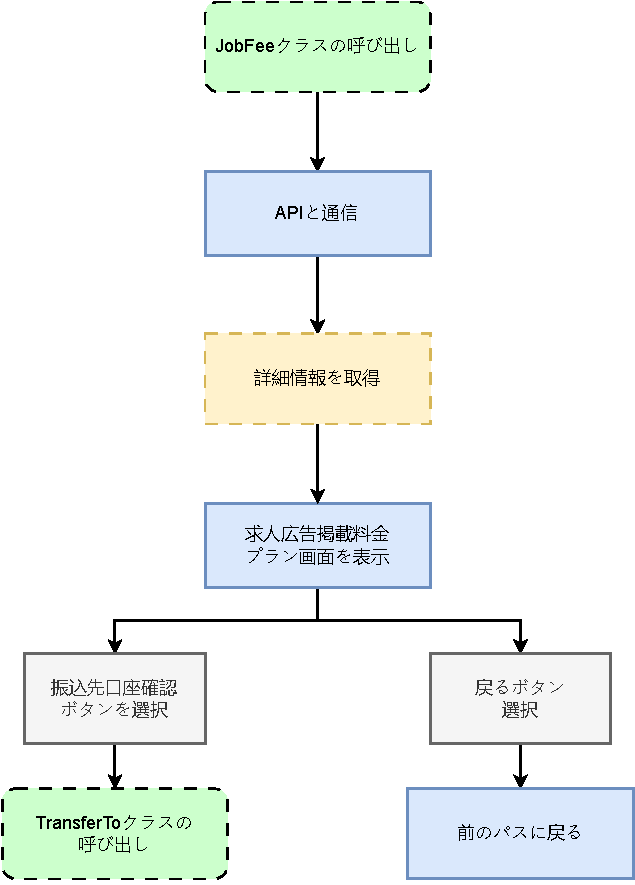
\includegraphics[width=11cm]{./images/internal-design/state_change_diagram/mypage/job_fee.pdf}
  \caption{job\_fee.dartの状態遷移図}
\end{figure}




\begin{table}[H]
  \centering
  \begin{tabular}{|c|l|l|} \hline
    モジュール名                & \multicolumn{2}{l|}{job\_fee\_select.dart}                                                               \\ \hline
    モジュール概要               & \multicolumn{2}{p{12cm}|}{求人掲載料金プランを選択する画面を表示するモジュール}                                                    \\ \hline
    責任者                   & \multicolumn{2}{l|}{新谷光城}                                                                                \\ \hline
    \multirow{7}{*}{構成要素} & クラス名                                                  & JobFeeSelect                                     \\ \cline{2-3}
                          & クラス種類                                                 & extends StatelessWidget                          \\ \cline{2-3}
                          & 処理概要                                                  & \multicolumn{1}{p{12cm}|}{求人掲載料金プラン選択画面を表示するクラス} \\ \cline{2-3}
                          & 入力                                                    & なし                                               \\ \cline{2-3}
                          & 出力                                                    & Widget                                           \\ \cline{2-3}
                          & \multicolumn{2}{l|}{他クラス・関数との関係}                                                                         \\ \cline{2-3}
                          & \multicolumn{2}{p{14cm}|}{
      change\_generalcorporation.dartのChangeGeneralCorporationプロバイダを組み込む
      \newline job\_fee\_select.dartのJobPostInfoプロバイダを組み込む
      \newline title\_appbar.dartのTitleAppBarクラスを組み込む
      \newline transfer\_to.dartのTransferToクラスを呼び出し振込口座確認画面を表示
      \newline event\_post\_write.dartのEventPostWriteクラスを呼び出しイベント広告掲載内容記述画面を表示
    \newline 戻るボタンの選択で前のモジュールに戻る}                                                                                                    \\ \hline
    \multirow{7}{*}{構成要素} & クラス名                                                  & JobPostInfo                                      \\ \cline{2-3}
                          & クラス種類                                                 & ChangeNotifier                                   \\ \cline{2-3}
                          & 処理概要                                                  & \multicolumn{1}{p{12cm}|}{求人広告投稿内容を保存しておくプロバイダ}  \\ \cline{2-3}
                          & 入力                                                    & なし                                               \\ \cline{2-3}
                          & 出力                                                    & なし                                               \\ \cline{2-3}
                          & \multicolumn{2}{l|}{他クラス・関数との関係}                                                                         \\ \cline{2-3}
                          & \multicolumn{2}{p{14cm}|}{なし}                                                                            \\ \hline
  \end{tabular}
\end{table}

\begin{figure}[H]
  \centering
  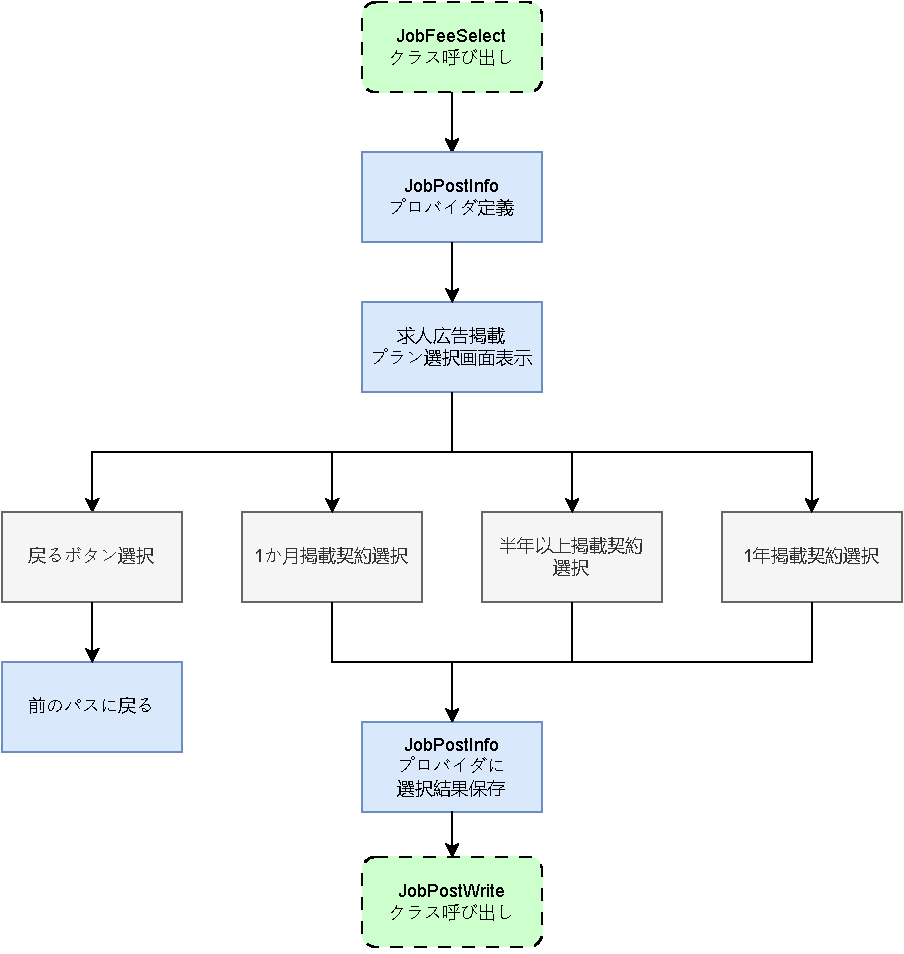
\includegraphics[width=17cm]{./images/internal-design/state_change_diagram/mypage/job_fee_select.pdf}
  \caption{job\_fee\_select.dartの状態遷移図}
\end{figure}


% \begin{table}[H]
%   \centering
%   \begin{tabular}{|c|l|l|} \hline
%     モジュール名                & \multicolumn{2}{l|}{post\_write\_comp.dart}                                                                            \\ \hline
%     モジュール概要               & \multicolumn{2}{p{12cm}|}{投稿したいと考えている内容が投稿時どのように見えるのかの確認を行う画面を表示するモジュール}                                               \\ \hline
%     責任者                   & \multicolumn{2}{l|}{新谷光城}                                                                                              \\ \hline
%     \multirow{7}{*}{構成要素} & クラス名                                                                     & PostWriteComp                               \\ \cline{2-3}
%                           & クラス種類                                                                    & extends StatelessWidget                     \\ \cline{2-3}
%                           & 処理概要                                                                     & \multicolumn{1}{p{12cm}|}{投稿内容確認画面を表示するクラス} \\ \cline{2-3}
%                           & 入力                                                                       & なし                                          \\ \cline{2-3}
%                           & 出力                                                                       & Widget                                      \\ \cline{2-3}
%                           & \multicolumn{2}{l|}{他クラス・関数との関係}                                                                                       \\ \cline{2-3}
%                           & \multicolumn{2}{p{14cm}|}{
%       change\_generalcorporation.dartのChangeGeneralCorporationプロバイダを組み込む
%       \newline job\_fee\_select.dartのJobPostInfoプロバイダを組み込む
%       \newline event\_fee\_select.dartのEventPostInfoプロバイダを組み込む
%       \newline title\_appbar.dartのTitleAppBarクラスを組み込む
%       \newline post\_conf.dartのPostConfクラスを呼び出し投稿確認オーバーレイを表示
%       \newline return\_write.dartのReturnWriteクラスを呼び出し必須内容記入漏れ注意オーバーレイを表示
%       \newline move\_conf.dartのMoveConfクラスを呼び出し投稿中に移動確認オーバーレイを表示
%     \newline 戻るボタンの選択で前のモジュールに戻る}                                                                                                                  \\ \hline
%   \end{tabular}
% \end{table}

% \begin{table}[H]
%   \centering
%   \begin{tabular}{|c|l|l|} \hline
%     モジュール名                & \multicolumn{2}{l|}{job\_post\_write.dart}                                                        \\ \hline
%     モジュール概要               & \multicolumn{2}{p{12cm}|}{イベント広告内容記述画面を表示するモジュール}                                                 \\ \hline
%     責任者                   & \multicolumn{2}{l|}{新谷光城}                                                                         \\ \hline
%     \multirow{7}{*}{構成要素} & クラス名                                              & JobPostWrite                                  \\ \cline{2-3}
%                           & クラス種類                                             & extends StatelessWidget                       \\ \cline{2-3}
%                           & 処理概要                                              & \multicolumn{1}{p{12cm}|}{求人広告内容記述画面を表示するクラス} \\ \cline{2-3}
%                           & 入力                                                & なし                                            \\ \cline{2-3}
%                           & 出力                                                & Widget                                        \\ \cline{2-3}
%                           & \multicolumn{2}{l|}{他クラス・関数との関係}                                                                  \\ \cline{2-3}
%                           & \multicolumn{2}{p{14cm}|}{
%       change\_generalcorporation.dartのChangeGeneralCorporationプロバイダを組み込む
%       \newline job\_fee\_select.dartのJobPostInfoプロバイダを組み込む
%       \newline title\_appbar.dartのTitleAppBarクラスを組み込む
%       \newline post\_conf.dartのPostConfクラスを呼び出し投稿確認オーバーレイを表示
%       \newline return\_write.dartのReturnWriteクラスを呼び出し必須内容記入漏れ注意オーバーレイを表示
%       \newline move\_conf.dartのMoveConfクラスを呼び出し投稿中に移動確認オーバーレイを表示
%     \newline 戻るボタンの選択で前のモジュールに戻る}                                                                                             \\ \hline
%   \end{tabular}
% \end{table}

% \begin{table}[H]
%   \centering
%   \begin{tabular}{|c|l|l|} \hline
%     モジュール名                & \multicolumn{2}{l|}{event\_post\_write.dart}                                                        \\ \hline
%     モジュール概要               & \multicolumn{2}{p{12cm}|}{イベント広告内容記述画面を表示するモジュール}                                                   \\ \hline
%     責任者                   & \multicolumn{2}{l|}{新谷光城}                                                                           \\ \hline
%     \multirow{7}{*}{構成要素} & クラス名                                              & EventPostWrite                                  \\ \cline{2-3}
%                           & クラス種類                                             & extends StatelessWidget                         \\ \cline{2-3}
%                           & 処理概要                                              & \multicolumn{1}{p{12cm}|}{イベント広告内容記述画面を表示するクラス} \\ \cline{2-3}
%                           & 入力                                                & なし                                              \\ \cline{2-3}
%                           & 出力                                                & Widget                                          \\ \cline{2-3}
%                           & \multicolumn{2}{l|}{他クラス・関数との関係}                                                                    \\ \cline{2-3}
%                           & \multicolumn{2}{p{14cm}|}{
%       change\_generalcorporation.dartのChangeGeneralCorporationプロバイダを組み込む
%       \newline event\_fee\_select.dartのEventPostInfoプロバイダを組み込む
%       \newline title\_appbar.dartのTitleAppBarクラスを組み込む
%       \newline post\_conf.dartのPostConfクラスを呼び出し投稿確認オーバーレイを表示
%       \newline return\_write.dartのReturnWriteクラスを呼び出し必須内容記入漏れ注意オーバーレイを表示
%       \newline move\_conf.dartのMoveConfクラスを呼び出し投稿中に移動確認オーバーレイを表示
%     \newline 戻るボタンの選択で前のモジュールに戻る}                                                                                               \\ \hline
%   \end{tabular}
% \end{table}

% \begin{table}[H]
%   \centering
%   \begin{tabular}{|c|l|l|} \hline
%     モジュール名                & \multicolumn{2}{l|}{not\_post\_list.dart}                                                                                    \\ \hline
%     モジュール概要               & \multicolumn{2}{p{12cm}|}{未振り込み投稿一覧画面を表示するモジュール}                                                                             \\ \hline
%     責任者                   & \multicolumn{2}{l|}{新谷光城}                                                                                                    \\ \hline
%     \multirow{7}{*}{構成要素} & クラス名                                                                     & NotPostList                                       \\ \cline{2-3}
%                           & クラス種類                                                                    & extends StatelessWidget                           \\ \cline{2-3}
%                           & 処理概要                                                                     & \multicolumn{1}{p{12cm}|}{未振り込み投稿一覧画面を動的に変更するクラス} \\ \cline{2-3}
%                           & 入力                                                                       & なし                                                \\ \cline{2-3}
%                           & 出力                                                                       & Widget                                            \\ \cline{2-3}
%                           & \multicolumn{2}{l|}{他クラス・関数との関係}                                                                                             \\ \cline{2-3}
%                           & \multicolumn{2}{p{14cm}|}{not\_post\_list.dartのNotPostListStateクラスを組み込む}                                                     \\ \hline
%     \multirow{7}{*}{構成要素} & クラス名                                                                     & NotPostListState                                  \\ \cline{2-3}
%                           & クラス種類                                                                    & extends StatelessWidget                           \\ \cline{2-3}
%                           & 処理概要                                                                     & \multicolumn{1}{p{12cm}|}{未振り込み投稿一覧画面の状態を返すクラス}   \\ \cline{2-3}
%                           & 入力                                                                       & なし                                                \\ \cline{2-3}
%                           & 出力                                                                       & State                                             \\ \cline{2-3}
%                           & \multicolumn{2}{l|}{他クラス・関数との関係}                                                                                             \\ \cline{2-3}
%                           & \multicolumn{2}{p{14cm}|}{
%       change\_generalcorporation.dartのChangeGeneralCorporationプロバイダを組み込む
%       \newline title\_appbar.dartのTitleAppBarクラスを組み込む
%       \newline event\_fee.dartのEventFeeクラスを呼び出しイベント広告掲載料金表示画面を表示
%       \newline job\_fee.dartのJobFeeクラスを呼び出し求人広告掲載料金表示画面を表示
%       \newline notpost\_delete\_confのNotpostDeleteConfクラスを呼び出し未投稿広告の削除確認画面を表示
%       \newline event\_post\_detail.dartのEventPostDetailクラスを呼び出し未投稿のイベント広告詳細画面を表示
%       \newline job\_post\_detail.dartのJobPostDetailクラスを呼び出し未投稿の求人広告詳細画面を表示
%     \newline 戻るボタンの選択で前のモジュールに戻る}                                                                                                                        \\ \hline
%   \end{tabular}
% \end{table}


\begin{table}[H]
  \centering
  \begin{tabular}{|c|l|l|} \hline
    モジュール名                & \multicolumn{2}{l|}{post\_mem\_list.dart}                                                                           \\ \hline
    モジュール概要               & \multicolumn{2}{p{12cm}|}{指定の求人広告に対しての応募者一覧を表示するレイヤー}                                                               \\ \hline
    責任者                   & \multicolumn{2}{l|}{新谷光城}                                                                                           \\ \hline
    \multirow{7}{*}{構成要素} & クラス名                                                                & PostMemList                                   \\ \cline{2-3}
                          & クラス種類                                                               & extends StatelessWidget                       \\ \cline{2-3}
                          & 処理概要                                                                & \multicolumn{1}{p{12cm}|}{応募者一覧画面を動的に変更するクラス} \\ \cline{2-3}
                          & 入力                                                                  & なし                                            \\ \cline{2-3}
                          & 出力                                                                  & Widget                                        \\ \cline{2-3}
                          & \multicolumn{2}{l|}{他クラス・関数との関係}                                                                                    \\ \cline{2-3}
                          & \multicolumn{2}{p{14cm}|}{post\_mem\_list.dartのPostMemListクラスを組み込む}                                                 \\ \hline
    \multirow{7}{*}{構成要素} & クラス名                                                                & PostMemListState                              \\ \cline{2-3}
                          & クラス種類                                                               & extends StatelessWidget                       \\ \cline{2-3}
                          & 処理概要                                                                & \multicolumn{1}{p{12cm}|}{応募者一覧画面の状態を返すクラス}   \\ \cline{2-3}
                          & 入力                                                                  & 応募者一覧リスト(List<Map<String, dynamic>>)          \\ \cline{2-3}
                          & 出力                                                                  & State                                         \\ \cline{2-3}
                          & \multicolumn{2}{l|}{他クラス・関数との関係}                                                                                    \\ \cline{2-3}
                          & \multicolumn{2}{p{14cm}|}{
      change\_generalcorporation.dartのChangeGeneralCorporationプロバイダを組み込む
      \newline title\_appbar.dartのTitleAppBarクラスを組み込む
      \newline apply\_conf.dartのApplyConfクラスを呼び出し応募者確認画面を表示
    \newline 戻るボタンの選択で前のレイヤーに戻る}                                                                                                                \\ \hline
  \end{tabular}
\end{table}

\begin{figure}[H]
  \centering
  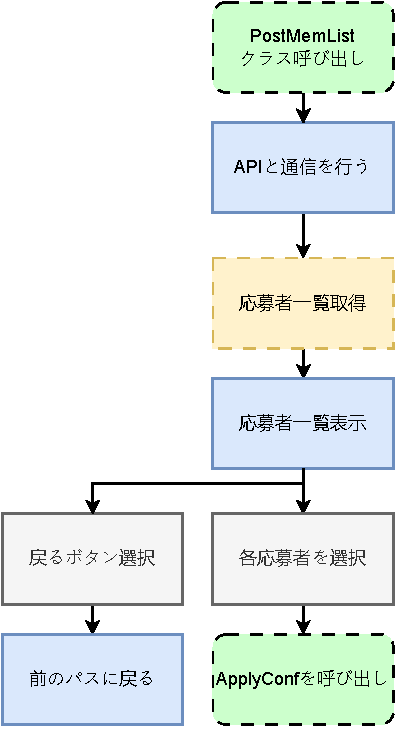
\includegraphics[width=7cm]{./images/internal-design/state_change_diagram/mypage/post_member_list.pdf}
  \caption{post\_mem\_list.dartの状態遷移図}
\end{figure}


\clearpage

\begin{table}[H]
  \centering
  \begin{tabular}{|c|l|l|} \hline
    モジュール名                & \multicolumn{2}{l|}{impressions.dart}                                                                                  \\ \hline
    モジュール概要               & \multicolumn{2}{p{12cm}|}{法人利用者が投稿を行った広告のインプレッション情報を閲覧できる画面を表示するモジュール}                                                 \\ \hline
    責任者                   & \multicolumn{2}{l|}{新谷光城}                                                                                              \\ \hline
    \multirow{7}{*}{構成要素} & クラス名                                                                   & Impressios                                    \\ \cline{2-3}
                          & クラス種類                                                                  & extends StatelessWidget                       \\ \cline{2-3}
                          & 処理概要                                                                   & \multicolumn{1}{p{12cm}|}{インプレッション画面を表示するクラス} \\ \cline{2-3}
                          & 入力                                                                     & Map$<$String, dynamic $>$ impressions         \\ \cline{2-3}
                          & 出力                                                                     & Widget                                        \\ \cline{2-3}
                          & \multicolumn{2}{l|}{他クラス・関数との関係}                                                                                       \\ \cline{2-3}
                          & \multicolumn{2}{p{14cm}|}{戻るボタンの選択で前のモジュールに戻る}                                                                         \\ \hline
  \end{tabular}
\end{table}

\begin{figure}[H]
  \centering
  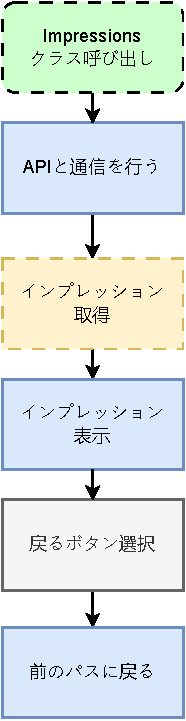
\includegraphics[width=4cm]{./images/internal-design/state_change_diagram/mypage/impressions.pdf}
  \caption{impressions.dartの状態遷移図}
\end{figure}

